\newif\ifieeeclass
\IfFileExists{IEEEtran.cls}{%
  \ieeeclasstrue\documentclass[10pt,journal]{IEEEtran}
}{%
  \ieeeclassfalse\documentclass[10pt,twocolumn]{article}
}

\usepackage{amsmath,amssymb}
\usepackage{booktabs}
\usepackage{tabularx}
\usepackage{graphicx}
\usepackage{float}
\IfFileExists{placeins.sty}{\usepackage{placeins}}{}
\IfFileExists{kotex.sty}{%
  \usepackage{kotex}
  \usepackage{fontspec}
  \setmainhangulfont{Noto Sans CJK KR}
  \setsanshangulfont{Noto Sans CJK KR}
}{%
  \usepackage{fontspec}
  \setmainfont{Noto Sans CJK KR}
  \setsansfont{Noto Sans CJK KR}
}
\usepackage{xcolor}
\usepackage{url}
\usepackage{xspace}
\usepackage{listings}
\usepackage[hidelinks]{hyperref}

\definecolor{safe}{RGB}{40,120,90}
\definecolor{guard}{RGB}{40,95,160}
\definecolor{warning}{RGB}{180,120,35}
\definecolor{unsafe}{RGB}{165,55,55}
\definecolor{neutral}{RGB}{70,70,70}

\newcolumntype{Y}{>{\raggedright\arraybackslash}X}
\newcolumntype{L}[1]{>{\raggedright\arraybackslash}p{#1}}
\newcommand{\coc}{CoC\xspace}
\newcommand{\sccoc}{Safety-Constrained CoC\xspace}
\newcommand{\vlm}{VLM\xspace}
\newcommand{\placeholder}[1]{%
  \fbox{\parbox[c][34mm][c]{0.94\linewidth}{\centering\small #1}}}

\renewcommand{\abstractname}{요약}
\ifieeeclass
  \renewcommand{\IEEEkeywordsname}{주요어}
\else
  \newenvironment{IEEEkeywords}{\par\small\noindent\textbf{주요어---}}{\par}
\fi
\renewcommand{\figurename}{그림}
\renewcommand{\tablename}{표}
\renewcommand{\refname}{참고문헌}

\renewcommand{\topfraction}{0.95}
\renewcommand{\bottomfraction}{0.90}
\renewcommand{\textfraction}{0.05}
\renewcommand{\floatpagefraction}{0.85}
\renewcommand{\dbltopfraction}{0.95}
\renewcommand{\dblfloatpagefraction}{0.85}
\setcounter{topnumber}{4}
\setcounter{bottomnumber}{3}
\setcounter{totalnumber}{6}
\setcounter{dbltopnumber}{3}
\makeatletter
\setlength{\@fptop}{0pt}
\setlength{\@dblfptop}{0pt}
\makeatother

\title{비전-언어 자율주행 모델의 안전성 향상을 위한 실행 가드:\\Safety-Constrained Chain-of-Causation}
\author{익명 저자}
\date{}

\begin{document}
\maketitle

\begin{abstract}
Alpamayo-R1과 같은 추론형 주행 VLM의 학습에서 Chain-of-Causation(CoC)은 장면 인식과 예측 궤적을 연결하는 중간 추론 신호로 활용된다. 그러나 "보행자에게 양보한다"와 같은 요구사항만으로는 정지선, 최소 간격 및 hold/release 등의 실행 한계가 정해지지 않는다. 본 논문은 CoC에 명시적 실행 가드를 결합한 Safety-Constrained CoC와, 동일 장면에서 계약만 바꾸는 paired-contract 벤치마크를 제안한다. 기존 CoC가 달성할 행동만 기술하는 데 비해, 본 방식은 그 행동이 언제 허용·금지·해제되는지까지 실행 조건으로 명시한다. 반복 실험에서 Safety-Constrained CoC는 기존 CoC 대비 가드 위반을 31.9\%에서 0\%로 줄이면서 목표 완료 성능을 유지했다. 가드 위반 감소는 정지·출발과 차선 변경 과제에서도 확인되었다. 이는 작은 VLM이 기존 CoC의 행동 목표를 유지하면서 추가된 실행 가드를 따르도록 학습될 수 있음을 보여준다. 다만 본 연구는 제한된 환경에서 궤적 후보 선택을 평가한 것으로, 실제 차량 환경에서의 효과와 안전성은 후속 검증이 필요하다.
\end{abstract}

\begin{IEEEkeywords}
자율주행, 비전-언어 모델, Chain-of-Causation, 자연어 안전 제약, 궤적 선택, 실행 가드
\end{IEEEkeywords}

\section{서론}
\label{sec:introduction}

종단 간(end-to-end, E2E) 자율주행은 카메라 영상과 자차 상태를 입력으로 받아 미래 궤적이나 제어 명령을 직접 예측한다 \cite{hu2023uniad,jiang2023vad}. 최근 비전-언어 모델(vision-language model, VLM)은 자연어 추론을 결합하여 장면에서 인식한 원인과 판단, 행동을 연결한다 \cite{sima2024drivelm,tian2024drivevlm}. Alpamayo-R1은 인과 연쇄(Chain-of-Causation, CoC)와 궤적을 함께 예측하는 대표적인 모델이다 \cite{wang2025alpamayo}. CoC는 "전방 차량 때문에 감속한다" 또는 "보행자에게 양보한다"처럼 특정 행동이 필요한 이유를 설명하므로, 궤적만 모방하는 학습보다 풍부한 학습 신호를 제공할 수 있다.

그러나 CoC가 행동의 이유와 목표를 설명하더라도 허용 가능한 궤적이 하나로 정해지는 것은 아니다. 예를 들어 "보행자에게 양보한 뒤 진행한다"는 요구사항만으로는 정지선을 넘지 않아야 하는지, 어느 정도의 감속도와 가가속도(jerk)를 허용할지, 상충 구역이 얼마나 오래 비어 있어야 출발할 수 있는지가 정해지지 않는다. 따라서 같은 목표를 달성하는 궤적 중에도 현재 실행 조건을 위반하는 궤적이 있을 수 있다. 반대로 지나치게 보수적인 궤적은 조건을 만족하더라도 불필요하게 진행을 멈출 수 있다.

본 논문은 기존 CoC가 일반적으로 잘못되었거나 위험하다고 주장하지 않는다. 대신 행동 목표를 설명하는 CoC에 실행 조건을 추가한 \sccoc{}를 제안한다. 요구사항은 무엇을 달성해야 하는지를 나타내고, 실행 가드는 언제 행동을 허용ㆍ금지ㆍ해제할지와 항상 지켜야 할 경계를 명시한다. 예를 들어 보행자 양보 요구사항에 "정지선을 넘지 않는다", "감속도와 가가속도의 상한을 지킨다", "상충 구역이 일정 시간 연속으로 비어 있을 때만 출발한다"는 가드를 추가할 수 있다.

\begin{figure*}[!t]
\centering
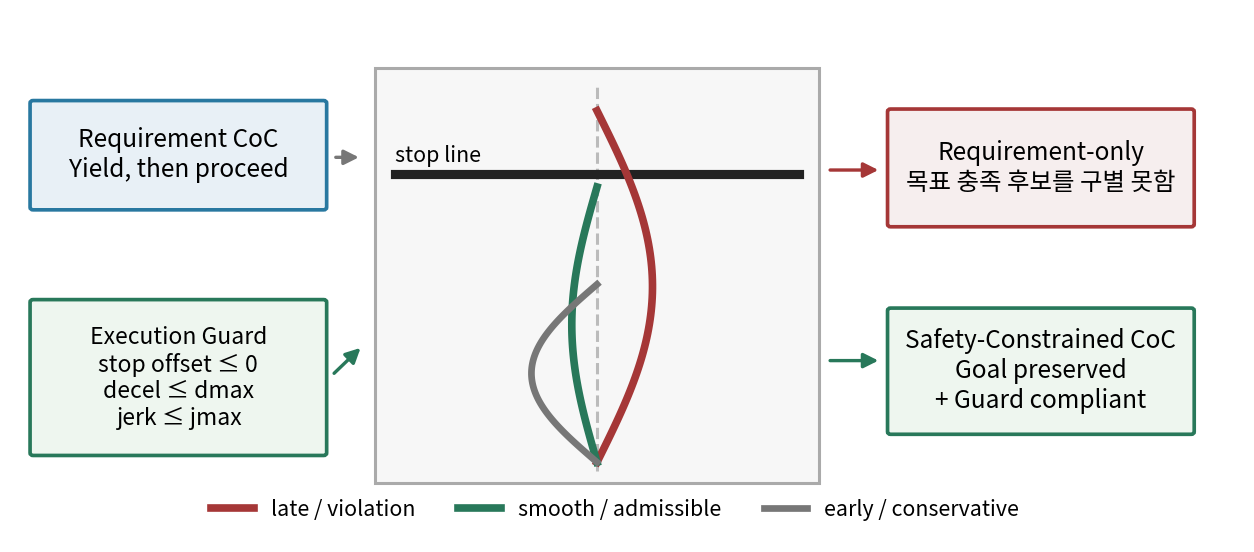
\includegraphics[width=0.98\textwidth]{figures/fig01_concept.png}
\caption{요구사항만 제시한 CoC와 실행 가드를 추가한 Safety-Constrained CoC의 비교.}
\label{fig:concept}
\end{figure*}

그림~\ref{fig:concept}은 동일한 "양보 후 진행" 목표를 달성하는 세 궤적 후보를 비교한다. 빨간색 궤적은 정지선이나 감속도ㆍ가가속도 제한을 위반하고, 회색 궤적은 필요 이상으로 일찍 정지하여 진행성을 잃는다. 반면 녹색 궤적은 행동 목표를 달성하면서 실행 가드도 만족한다. 요구사항만 포함한 CoC는 이 후보들을 명확히 구분하기 어렵지만, Safety-Constrained CoC는 목표를 유지하면서 허용 가능한 궤적을 선택할 기준을 제공한다.

제안한 가드가 궤적 선택에 실제로 영향을 주는지 확인하기 위해 같은 장면, 같은 행동 목표 및 같은 궤적 후보를 사용하되 실행 조건만 다른 두 문제를 한 쌍으로 구성한다. 이를 쌍대 계약(paired-contract) 벤치마크라 한다. 한 문제는 더 자유로운 행동을 허용하고 다른 문제는 안전 조건을 더 엄격하게 적용하므로, 두 문제에서 선택해야 할 궤적이 달라진다. 따라서 장면만 외운 모델은 두 문제를 모두 맞힐 수 없으며, 제시된 가드를 읽고 판단해야 한다. 또한 모든 후보가 기본 행동 목표는 달성하도록 구성하여, 성능 차이가 목표 인식이 아니라 가드 준수에서 발생하도록 했다.

본 논문의 연구 질문은 다음과 같다.
\begin{enumerate}
    \item \textbf{RQ1 효과:} \sccoc{}는 요구사항만 포함한 CoC보다 가드를 위반하는 궤적의 선택을 줄이는가?
    \item \textbf{RQ2 목표 보존:} 가드 위반의 감소가 항상 정지하거나 교착되는 방식이 아니라, 행동 목표를 완료하면서 나타나는가?
    \item \textbf{RQ3 적용 범위:} 이러한 효과가 정적 후보 선택, 시간에 따른 유지ㆍ해제, 정지 및 차선 변경 상황에서도 반복되는가?
    \item \textbf{RQ4 일반화:} 표현 변형, 학습에서 보지 못한 수치, 부정문, 경계값 및 단위 변환에서도 효과가 유지되는가?
\end{enumerate}

본 논문의 기여는 다음과 같다.
\begin{enumerate}
    \item 행동의 이유와 목표를 설명하는 CoC에 실행 가드를 결합한 \sccoc{}를 제안한다.
    \item 동일한 장면에서 실행 조건만 바꾸는 쌍대 계약 평가와, 행동 목표는 달성하지만 가드를 위반하는 반례 구성 방법을 제시한다.
    \item 가드 위반, 목표 완료, 교착, 과도한 보수성 및 계약 쌍의 정확도를 함께 측정하는 평가 체계를 구성한다.
    \item 정적ㆍ시간적ㆍ복합 주행 과제에서 소형 VLM이 가드에 따라 궤적 후보를 선택하도록 학습될 수 있음을 세 가지 난수 초기값으로 검증한다.
    \item 추가 학습 없이 Alpamayo-R1의 반응을 진단하고, 고난도 및 폐루프 보조 실험을 통해 입력 문장에 대한 반응, 학습 후 준수 및 실행 중 강제 적용의 차이를 분석한다.
\end{enumerate}

본 연구는 합성 이미지와 설명으로 제시된 궤적 후보를 사용하여 소형 VLM의 학습 가능성을 평가한다. 따라서 실제 차량의 충돌 감소, Alpamayo-R1을 학습한 뒤의 성능 향상 또는 완전한 도로 안전 명세를 입증하지는 않는다.

\section{관련 연구}
\label{sec:related}

\subsection{추론 보강형 E2E/VLA 자율주행}

DriveLM은 주행 장면을 그래프 기반 시각 질의응답으로 구조화하고 \cite{sima2024drivelm}, DriveVLM은 VLM의 장면 이해와 계획을 결합한다 \cite{tian2024drivevlm}. Alpamayo-R1은 CoC 추론과 행동/궤적 예측을 연결하여 긴 꼬리 상황에서의 일반화를 목표로 한다 \cite{wang2025alpamayo}. 한편 자율주행 VLM의 신뢰성 연구는 장면 이해와 행동 추론의 평가 지표 및 데이터 품질 문제를 지적한다 \cite{xie2025drivebench}. 본 연구는 객체 환각이나 CoC의 일반적 사실 오류를 다시 검출하기보다, 동일한 행동 목표를 달성하는 후보 안에서 명시된 허용조건을 학습하고 적용할 수 있는지를 다룬다.

\subsection{주행 안전 제약과 검증}

자율주행 안전 연구는 안전거리, 책임 민감 안전 모델, 도달 가능성, runtime monitor와 shield처럼 실행 단계에서 제약을 검사하는 방법을 발전시켜 왔다 \cite{shalev2017rss,katz2019marabou}. 시나리오 명세 및 폐루프 시험은 보지 않은 조합에서 학습 정책의 취약성을 발견하는 데 사용된다 \cite{fremont2019scenic,zhang2023cat}. 이러한 방법은 정밀한 제약 집행에 적합하지만 자연어 reasoning과 실행 계약 사이의 인터페이스는 별도 문제다.

\subsection{자연어와 정형 명세의 역할}

자연어는 사전학습 VLM이 처리하기 쉬우며 사람에게 편리하지만, 부정 범위, 단위 및 경계 연산자가 모호할 수 있다. 정형 명세는 정확한 판정과 runtime enforcement에 적합하지만 기반 VLM이 임의 논리 문법을 즉시 실행할 것이라고 가정할 수 없다. 본 논문은 두 표현을 경쟁 관계로 두지 않는다. 자연어 \sccoc{}를 학습 인터페이스로 평가하고, 수치 판정은 독립 verifier로 계산한다. 자연어에서 typed contract로의 컴파일은 후속 연구로 남긴다.

\subsection{차별점}

본 연구는 사고 trajectory를 필요로 하지 않는다. 모든 후보가 CoC 목표를 달성하지만 가드 준수 여부와 진행도가 다르도록 구성한다. 또한 동일 장면의 계약만 바꾸는 counterfactual pair와 shuffled constraint 통제를 사용하고, 위반 감소와 목표 완료를 동시에 평가한다.

\section{문제 정의}
\label{sec:problem}

장면 입력을 $x$, 요구사항을 기술한 CoC를 $R$, 실행 가드를 $G$, 궤적 후보 집합을 $\mathcal{T}(x)=\{\tau_1,\ldots,\tau_K\}$라 하자. $\mathrm{Goal}(\tau,R)$는 후보가 요구사항의 행동 목표를 완료하는지, $\mathrm{Sat}(\tau,G)$는 후보가 실행 가드를 만족하는지를 나타낸다. 궤적의 진행도 또는 효용은 $U(\tau)$로 둔다. 본 연구의 선택 목표는 다음과 같다.
\begin{equation}
\begin{aligned}
\tau^*&=\arg\max_{\tau\in\mathcal{T}(x)} U(\tau),\\
\mathrm{s.t.}\quad &\mathrm{Goal}(\tau,R)=1,\quad \mathrm{Sat}(\tau,G)=1.
\end{aligned}
\label{eq:selection}
\end{equation}

$\mathrm{Goal}=1$이지만 $\mathrm{Sat}=0$인 후보는 행동 목표를 달성하더라도 현재 실행 조건을 위반하는 반례다. 반대로 가드를 위반하지 않지만 목표를 완료하지 못하는 후보는 교착 후보로 구분한다. 따라서 항상 정지하는 정책은 가드 위반률이 낮더라도 바람직한 정책으로 볼 수 없다.

\begin{table}[t]
\centering
\caption{Safety-Constrained CoC의 실행 가드 유형.}
\label{tab:taxonomy}
\footnotesize
\begin{tabularx}{\columnwidth}{L{0.30\columnwidth}Y}
\toprule
유형 & 의미와 예 \\
\midrule
활성화(Activation) & 보행자가 상충 구역에 들어오면 양보 의무 활성화 \\
불변 조건(Invariant) & 의무가 활성화된 동안 정지선 통과 금지 \\
수치 경계(Bound) & 차량 간격 $\geq6$ m, 감속도 $\leq4$ m/s$^2$ \\
금지 조건(Prohibition) & 차량 간격이 기준 미만이면 차선 변경 계속 금지 \\
해제 조건(Release) & 상충 구역이 1.5초 연속으로 비면 출발 허용 \\
대체 동작(Fallback) & 관측이 불확실하면 정지 상태 유지 \\
종료 조건(Termination) & 안전 간격을 유지한 상태에서 차선 변경 완료 \\
\bottomrule
\end{tabularx}
\end{table}

\subsection{표 1로부터 S-C CoC 구성}

표~\ref{tab:taxonomy}는 하나의 완성된 안전 명세가 아니라 장면과 행동 목표에 따라 선택하는 실행 가드의 구성 요소를 제시한다. 표에 정리된 일곱 가지 가드 유형의 집합을 $\mathcal{G}_{\mathrm{tax}}$라 하고, 장면 $x$와 요구사항 $R$에 필요한 가드의 부분집합을 $\mathcal{S}(x,R)$라 하면, 실행 가드와 S-C CoC의 구성 관계는 다음과 같이 나타낼 수 있다.
\begin{equation}
\begin{aligned}
\mathcal{S}(x,R)&\subseteq\mathcal{G}_{\mathrm{tax}},\\
G(x,R)&=\bigwedge_{g\in\mathcal{S}(x,R)}g,\\
\mathrm{SCCoC}(x,R)&=R\oplus G(x,R).
\end{aligned}
\label{eq:sccoc-compose}
\end{equation}
여기서 $\oplus$는 행동 요구사항과 선택된 가드 문장을 하나의 S-C CoC로 결합함을 뜻한다. 표의 모든 유형을 항상 사용하는 것은 아니며, 장면과 목표에 관련된 조건만 선택한다.

\paragraph{보행자 양보 예.}
기본 CoC가 "보행자에게 양보한 뒤 진행한다"라면 활성화, 불변 조건, 수치 경계, 해제 조건 및 대체 동작을 선택할 수 있다. 이때 표~\ref{tab:taxonomy}로부터 다음 S-C CoC를 구성할 수 있다.
\begin{quote}
\small
보행자가 상충 구역에 있으면 양보 의무를 활성화한다. 의무가 활성화된 동안 정지선을 넘지 않고 감속도를 $4\,\mathrm{m/s^2}$ 이하로 유지한다. 관측이 불확실하면 정지 상태를 유지한다. 상충 구역이 1.5초 이상 연속으로 비어 있을 때만 의무를 해제하고 출발한다.
\end{quote}
이 문장은 단순히 "양보한다"는 목표뿐 아니라 정지 위치, 감속 한계, 불확실할 때의 행동 및 출발 허용 시점을 함께 규정한다.

\paragraph{차선 변경 예.}
기본 CoC가 "안전하게 목표 차선으로 이동한다"라면 수치 경계, 금지 조건, 해제 조건 및 종료 조건을 선택할 수 있다. 구성된 S-C CoC는 다음과 같다.
\begin{quote}
\small
목표 차선의 차량 간격이 6 m 미만이면 차선 변경을 계속하지 않는다. 안전 간격이 다시 확보되면 차선 변경을 재개할 수 있다. 목표 차선에 진입한 뒤 안전 간격이 유지될 때 차선 변경을 완료한다.
\end{quote}
이 예에서는 같은 차선 변경 목표라도 차량 간격에 따라 계속 진행, 중단, 재개 및 완료 시점이 달라진다.

표~\ref{tab:taxonomy}만으로 장면에 필요한 S-C CoC가 자동으로 결정되는 것은 아니다. 장면에서 관측 가능한 상태와 기본 CoC의 행동 목표를 함께 사용하여 관련 가드를 선택해야 한다. 따라서 본 연구의 가드는 현재 데이터와 궤적 후보에서 측정 가능한 실행 의무를 구조화한 부분 계약이며, 완전한 도로 안전 명세를 의미하지 않는다.

\raggedbottom
\section{Safety-Constrained CoC와 평가 방법}
\label{sec:method}

본 장의 목적은 모델이 실행 가드를 실제로 읽고 궤적 선택에 사용하는지 확인하는 방법을 설명하는 것이다. 이를 분명하게 측정하기 위해 모델이 새로운 궤적을 직접 만들게 하지 않고, 미리 만든 여러 후보 중 하나를 고르게 한다. 모델이 직접 궤적을 만들면 궤적 생성 능력과 가드 이해 능력이 결과에 함께 섞인다. 후보 선택 문제로 범위를 좁히면, 같은 후보를 놓고 가드가 바뀔 때 모델의 선택도 바뀌는지를 직접 확인할 수 있다.

\subsection{제안 방법의 전체 흐름}

그림~\ref{fig:pipeline}의 과정은 세 단계로 이루어진다. 첫째, 모델에 장면 이미지, 기본 CoC, 실행 가드와 궤적 후보를 준다. 기본 CoC는 "보행자에게 양보한 뒤 진행한다"처럼 달성할 행동을 말한다. 실행 가드는 "정지선을 넘지 않는다" 또는 "차량이나 보행자의 이동 경로가 겹치는 구역이 1.5초 동안 비어 있을 때만 출발한다"처럼 그 행동을 언제, 어느 범위에서 허용할지를 정한다. 각 후보에는 정지 위치, 속도, 감속도, 가가속도(가속도가 변하는 정도), 차량 간격과 진입 시점이 함께 적혀 있다.

둘째, 모델은 이미지와 문장을 읽고 후보 하나를 선택한다. 셋째, 모델과 분리된 검증기(verifier)가 선택된 후보의 수치를 다시 계산한다. 예를 들어 정지선을 넘었는지, 최소 간격을 지켰는지, 필요한 시간만큼 기다렸는지를 확인한다. 따라서 모델이 스스로 "안전하다"고 답한 것만으로 정답으로 인정하지 않는다. 모델의 선택과 검증기의 계산 결과가 모두 맞아야 가드를 지킨 선택으로 판정한다.

\begin{figure*}[!t]
\centering
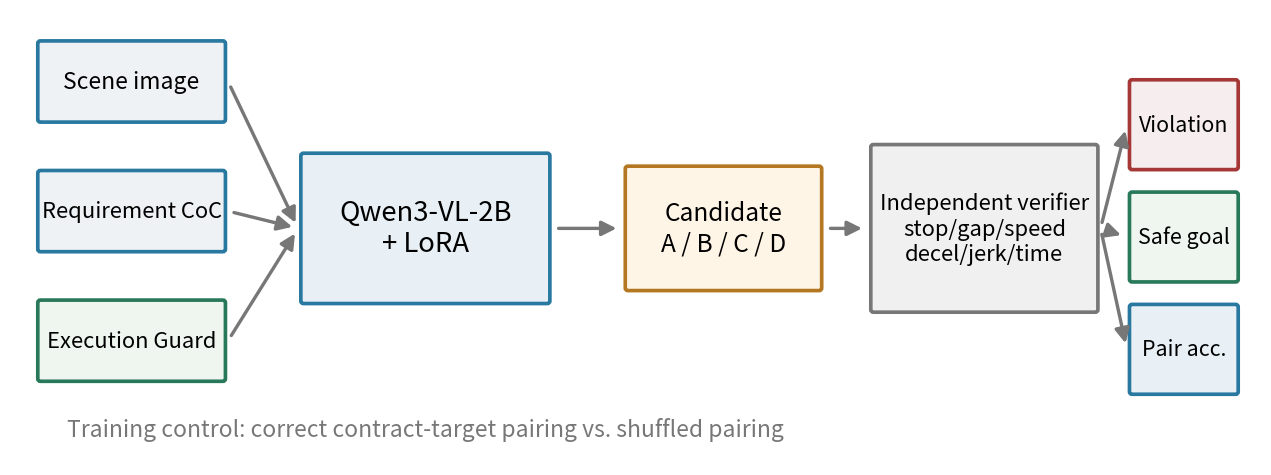
\includegraphics[width=0.98\textwidth]{figures/fig02_pipeline.png}
\caption{Safety-Constrained CoC의 입력, 궤적 후보 선택 및 독립 검증 과정. 모델은 후보 하나를 선택하고, 별도의 검증기가 선택된 후보의 목표 달성과 가드 준수를 판정한다.}
\label{fig:pipeline}
\end{figure*}

\subsection{CoC와 실행 가드의 입력 방식}

본 연구는 기본 CoC에 실행 가드를 결합한 형식을 제안한다. 예를 들어 기본 CoC가 "횡단보도 앞 보행자에게 양보한 뒤, 허용되면 진행한다"라면 다음 조건을 덧붙일 수 있다.

\begin{quote}\small
정지선을 넘지 않는다. 최대 감속도는 $3.8\,\mathrm{m/s^2}$, 최대 가가속도는 $5.0\,\mathrm{m/s^3}$를 넘지 않는다. 상충 구역이 정해진 시간 동안 비어 있을 때만 출발한다.
\end{quote}

이 실행 가드를 기본 CoC 뒤에 이어서 한 문장 묶음으로 제시한 방식을 \textbf{CoC 통합형}이라 한다. 모델은 이 입력에서 "무엇을 해야 하는가"와 "그 행동을 언제 허용하는가"를 함께 읽는다. 다만 성능이 좋아지더라도 그 이유가 가드의 의미를 배웠기 때문인지, 단순히 문장이 더 길어졌기 때문인지 구분해야 한다. 이를 위해 표~\ref{tab:representations}의 다섯 방식을 비교한다.

\begin{table*}[!t]
\centering
\caption{CoC와 실행 가드를 모델에 제시하는 다섯 가지 방식.}
\label{tab:representations}
\footnotesize
\begin{tabularx}{\textwidth}{L{0.19\textwidth}L{0.25\textwidth}Y}
\toprule
조건 & 모델에 주는 정보 & 비교 목적 \\
\midrule
요구사항 전용형 & 기본 CoC만 제시 & 실행 가드가 없을 때 장면과 행동 목표만으로 후보를 고르는 기준선 \\
CoC 통합형 & 기본 CoC 뒤에 실행 가드를 이어서 제시 & 요구사항과 실행 조건을 한 문맥에서 함께 학습하는 제안 조건 \\
가드 분리형 & 기본 CoC와 실행 가드를 서로 다른 항목으로 제시 & 같은 내용을 분리해서 제시했을 때의 차이 확인 \\
대응을 섞은 가드 & 가드 문장은 주지만 학습할 때 정답 후보와의 대응을 바꿈 & 문장이 추가된 효과와 올바른 가드 의미를 학습한 효과를 구분 \\
논리식 가드 & 실행 조건을 정해진 논리식으로 제시 & 자연어가 아닌 구조화된 표현을 현재 모델이 처리할 수 있는지 확인 \\
\bottomrule
\end{tabularx}
\end{table*}

특히 "대응을 섞은 가드"는 문장의 길이와 의미의 효과를 나누어 보기 위한 조건이다. 이 조건에도 가드 문장은 들어 있지만, 학습할 때 가드와 정답 후보를 일부러 잘못 연결한다. CoC 통합형은 잘 맞고 이 조건은 맞지 않는다면, 단순히 문장이 추가되어서가 아니라 올바른 가드-행동 관계를 배웠다고 해석할 수 있다. "논리식 가드"는 자연어 대신 정해진 기호 형식으로 같은 조건을 준다. 이 비교는 자연어와 논리식 중 어느 쪽이 본질적으로 우수한지 판정하려는 것이 아니라, 현재 VLM과 학습 방법이 두 표현을 얼마나 잘 처리하는지 확인하기 위한 것이다.

\subsection{같은 장면에서 실행 조건만 바꾸는 평가}

한 장면으로 정답이 서로 다른 두 문제를 만든다. 두 문제에는 같은 이미지, 같은 CoC 목표와 같은 궤적 후보를 사용한다. 바꾸는 것은 실행 가드뿐이다. 가드가 달라지면 올바른 후보도 달라지게 구성한다. 따라서 모델이 두 문제를 모두 맞히려면 장면만 보고 같은 답을 반복해서는 안 되고, 가드를 읽은 뒤 선택을 바꾸어야 한다. 이 두 문제의 묶음을 \textbf{쌍대 계약(paired-contract)}이라 한다.

그림~\ref{fig:pair}은 차선 변경 예에서 무엇이 고정되고 무엇이 바뀌는지를 보여준다. 두 계약 모두 현재 차량 간격은 7.2 m이며 후보도 같다. 후보 A는 현재 간격에서 바로 차선을 변경하고, 후보 B는 차선 변경을 중단한 뒤 필요한 간격이 확보되면 다시 시도한다. 최소 간격이 5.5 m인 완화 계약에서는 $7.2 \geq 5.5$이므로 후보 A가 허용되고 진행도가 높은 후보 A를 선택한다. 반면 최소 간격이 9.0 m인 엄격 계약에서는 $7.2 < 9.0$이므로 후보 A가 가드를 위반하고 후보 B를 선택해야 한다.

즉, 완화 계약과 엄격 계약은 장면이 아니라 허용 기준만 다르다. 모델이 두 문제에 같은 후보를 답하면 적어도 하나는 틀린다. "계약 전환 쌍 정확도"는 두 문제를 모두 맞혔을 때만 그 쌍을 정답으로 계산한다. 이 값이 높을수록 모델이 최소 간격의 변화를 읽고 선택에 반영했다고 볼 수 있다.

\begin{figure*}[!t]
\centering
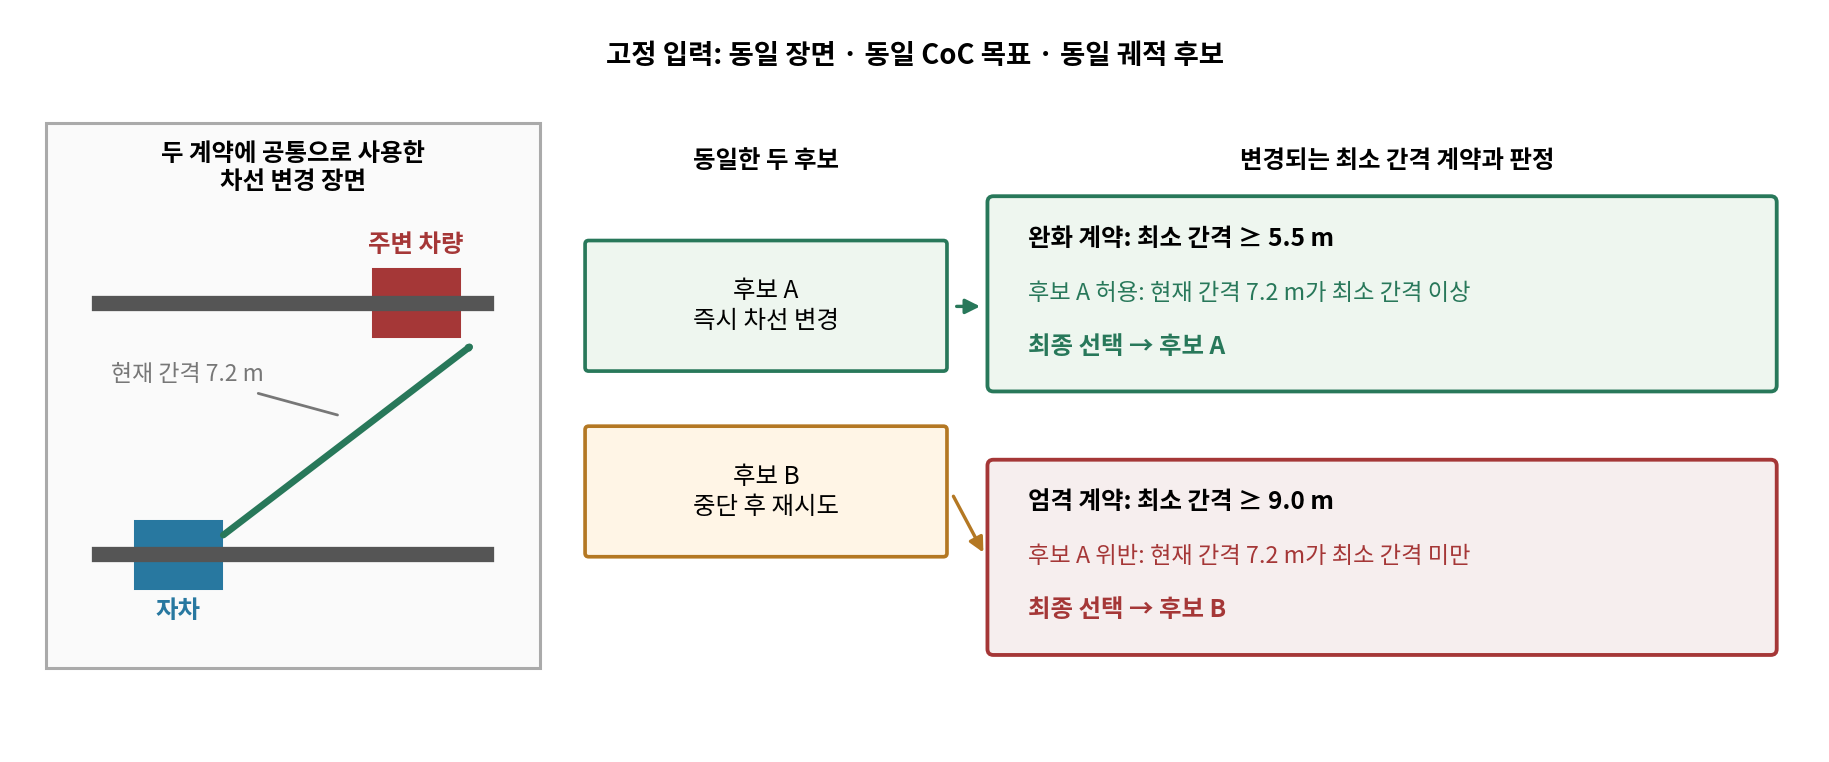
\includegraphics[width=0.98\textwidth]{figures/fig03_paired_contract.png}
\caption{쌍대 계약의 차선 변경 예. 장면, CoC 목표, 현재 간격 7.2 m 및 후보 A/B는 고정하고 최소 간격만 5.5 m에서 9.0 m로 바꾼다. 완화 계약에서는 즉시 차선 변경하는 후보 A가 허용되지만, 엄격 계약에서는 같은 후보가 최소 간격을 위반하므로 중단 후 재시도하는 후보 B를 선택한다.}
\label{fig:pair}
\end{figure*}

시간 과제에서는 행동이 다른 네 후보를 사용한다. 모델은 $A$, $B$, $C$, $D$ 중 하나를 답하지만, 이 문자는 후보를 구별하기 위한 이름일 뿐이다. 예를 들어 $A$가 언제나 조기 진입을 뜻하는 것은 아니다. 표~\ref{tab:candidate-roles}은 후보가 실제로 수행하는 네 가지 행동을 보여준다.

\begin{table*}[!t]
\centering
\caption{시간 과제의 네 궤적 역할과 계약에 따른 판정 예.}
\label{tab:candidate-roles}
\footnotesize
\begin{tabularx}{\textwidth}{L{0.18\textwidth}L{0.29\textwidth}L{0.20\textwidth}Y}
\toprule
궤적 역할 & 행동 & 완화 계약 & 엄격 계약 \\
\midrule
조기 진입 & 상충 구역이 비기 전에 진입 & 가드 위반 & 가드 위반 \\
짧은 대기 후 진입 & 상충 구역이 빈 뒤 짧게 기다리고 진행 & 선택 가능 & 대기시간 부족으로 위반 \\
긴 대기 후 진입 & 충분한 확인 시간을 거친 뒤 진행 & 허용되지만 진행이 느림 & 목표를 완료하는 적절한 후보 \\
계속 정지 & 평가 시간이 끝날 때까지 정지 & 목표 미완료 또는 교착 & 목표 미완료 또는 교착 \\
\bottomrule
\end{tabularx}
\end{table*}

한 장면에서는 $A$가 조기 진입이고 $B$가 짧은 대기일 수 있다. 다음 장면에서는 문자와 행동의 대응을 바꾸어 $A$가 긴 대기를 나타내게 할 수 있다. 이렇게 하면 모델이 항상 같은 문자만 고르는 방법으로 정답을 외울 수 없다. 정적 실험은 두 후보 $A/B$를, 시간 및 다중 주행 실험은 네 후보 $A/B/C/D$를 사용한다. 어느 실험에서도 특정 문자가 항상 안전하거나 항상 위험한 행동을 뜻하지 않는다.

\subsection{모델 학습과 정답 후보 생성}

기반 모델은 Qwen3-VL-2B-Instruct이다. 전체 모델을 다시 학습하지 않고 일부 추가 매개변수만 조정하는 LoRA 방식을 사용한다. 모델이 한 번에 받는 학습 자료는 다음 다섯 부분으로 구성된다.

\begin{enumerate}
\item 장면을 나타내는 합성 이미지,
\item 달성해야 할 행동을 설명하는 기본 CoC,
\item 실험 조건에 따른 실행 가드,
\item 각 후보의 행동과 측정값을 적은 설명,
\item 허용되는 후보 중 진행도가 가장 높은 후보를 고르라는 지시.
\end{enumerate}

모델은 후보 문자 하나를 답한다. 정답은 다음 세 단계로 정한다. 먼저 CoC의 행동 목표를 끝내지 못한 후보를 제외한다. 그다음 실행 가드를 위반한 후보를 제외한다. 마지막으로 남은 후보 중에서 가장 원활하게 진행하는 후보를 정답으로 삼는다. 모든 장면에는 목표와 가드를 함께 만족하는 후보가 적어도 하나 있다. 이는 식~\eqref{eq:selection}을 학습 자료 생성에 그대로 적용한 것이다.

예를 들어 가장 빨리 진행하는 후보가 최소 간격을 위반하면 정답이 될 수 없다. 반대로 가드 위반을 피하기 위해 끝까지 정지하는 후보도 행동 목표를 완료하지 못하므로 정답이 아니다. 모델은 "진행"과 "가드 준수"를 동시에 만족하는 후보를 찾아야 한다.

\subsection{독립 궤적 검증과 평가 지표}

모델의 답은 $A$와 같은 후보 문자일 뿐이다. 이 답이 실제로 가드를 지켰는지는 별도 검증기가 계산한다. 검증기는 표~\ref{tab:verifier-fields}의 수치를 후보 데이터에서 읽고 가드의 기준과 직접 비교한다. 예를 들어 최소 간격이 9.0 m라면 선택한 후보의 간격이 9.0 m 이상인지 확인한다.

\begin{table}[t]
\centering
\caption{독립 검증기가 확인하는 주요 값.}
\label{tab:verifier-fields}
\footnotesize
\begin{tabularx}{\columnwidth}{L{0.34\columnwidth}Y}
\toprule
확인 값 & 판정 예 \\
\midrule
정지선 기준 위치 & 0 m보다 크면 정지선을 넘어선 것으로 판정 \\
최대 속도 & 허용된 속도 상한을 넘는지 확인 \\
최대 감속도 & 급격한 감속 한계를 넘는지 확인 \\
최대 가가속도 & 가속도 변화가 허용 한계를 넘는지 확인 \\
최소 차량 간격 & 다른 차량과 필요한 거리를 유지하는지 확인 \\
교차로 진입 시점 & 상충 구역이 빈 뒤 필요한 대기시간을 지켰는지 확인 \\
\bottomrule
\end{tabularx}
\end{table}

표~\ref{tab:method-metrics}은 평가에 사용한 지표를 정리한다. 이 가운데 "가드 준수 목표 완료율"은 두 가지를 동시에 만족한 비율이다. 첫째, 선택한 후보가 CoC의 행동 목표를 완료해야 한다. 둘째, 실험에서 제시한 실행 가드를 모두 지켜야 한다. 이 지표는 실제 도로의 모든 위험이 제거되었다는 뜻은 아니다.

\begin{table}[t]
\centering
\caption{주요 평가 지표와 의미.}
\label{tab:method-metrics}
\footnotesize
\begin{tabularx}{\columnwidth}{L{0.31\columnwidth}Y}
\toprule
지표 & 의미 \\
\midrule
후보 정확도 & 모델이 데이터 생성 규칙으로 정한 최적 후보를 선택한 비율 \\
가드 위반률 & 선택한 후보가 하나 이상의 실행 가드를 위반한 비율 \\
가드 준수 목표 완료율 & 선택한 후보가 실행 가드를 지키면서 기본 CoC의 행동 목표도 완료한 비율 \\
교착률 & 가드를 위반하지 않지만 계속 정지하여 행동 목표를 완료하지 못한 비율 \\
과도한 보수 선택률 & 가드는 지키지만 같은 계약에서 허용되는 더 높은 진행도의 후보가 있는데도 지나치게 느린 후보를 고른 비율 \\
계약 전환 쌍 정확도 & 같은 장면의 완화 계약과 엄격 계약을 모두 맞힌 쌍의 비율 \\
\bottomrule
\end{tabularx}
\end{table}

일반 후보 정확도는 두 문제 중 하나만 맞혀도 각각의 정답으로 센다. 반면 계약 전환 쌍 정확도는 완화 계약과 엄격 계약을 모두 맞혀야 1로 센다. 따라서 이 지표는 모델이 가드가 바뀔 때 후보 선택도 바꾸었는지를 더 엄격하게 보여준다.

\subsection{학습된 가드 준수와 실제 실행 안전의 구분}

본 연구가 확인하는 것은 모델이 주어진 후보 중에서 가드를 지키는 후보를 더 잘 고를 수 있는가이다. 이것은 실제 차량에서 충돌을 막는 안전 보장과 다르다. 여기서 사용한 검증기는 실험 결과를 계산하는 도구이며, 차량의 명령을 실시간으로 막거나 수정하는 차단 장치가 아니다.

실제 차량에 적용하려면 두 단계가 더 필요하다. 먼저 자연어 가드에서 조건의 종류, 비교 방향, 수치, 단위와 조건을 지킬 수 없을 때의 대체 행동을 정확히 추출해야 한다. 예를 들어 "최소 간격 9 m"를 "거리, 이상, 9, m"처럼 일정한 형식으로 바꾸고 단위도 통일해야 한다. 다음으로 모델이 만든 궤적을 독립 검증기나 실행 차단 장치가 다시 검사해야 한다. 따라서 본 연구는 제한된 후보 선택 과제에서 가드 준수를 학습할 수 있음을 보일 뿐, 실제 도로의 완전한 안전 명세나 차량 안전을 보장하지 않는다.

\section{실험 및 결과}
\label{sec:experiments}

실험은 앞 실험에서 확인된 한계를 다음 실험이 보완하는 순서로 진행한다. 먼저 추가 학습을 하지 않은 Alpamayo-R1이 가드 문장에 반응하는지 확인한다. 그다음 작은 VLM을 학습하여 가드와 행동의 관계 자체를 배울 수 있는지 살펴본다. 이 과정에서 단순한 정지/진행 문제는 장면만 보고도 답을 맞힐 수 있다는 한계가 드러난다. 이를 해결하기 위해 이후 실험에서는 같은 장면과 같은 행동 목표를 유지하고 가드만 바꾸어 정답이 달라지게 한다. 평가 범위도 정적 경계, 대기와 출발의 시간 조건, 정지와 차선 변경 순으로 넓힌다. 마지막 폐루프 실험에서는 학습된 가드만으로 충분한지, 실행 중에 별도 차단 장치가 필요한지를 살펴본다.

이 장에서 사용하는 "가드 준수 목표 완료"는 실험에서 제시한 가드를 지키면서 CoC의 행동 목표까지 끝냈다는 뜻이다. 실제 도로의 모든 위험이 제거되었다는 뜻은 아니다. 전체 실험의 질문과 대표 결과는 표~\ref{tab:suite}에 먼저 요약하였다.

\subsection{Alpamayo-R1 사전학습 상태 진단}

\paragraph{확인 목적.}
첫 실험의 질문은 간단하다. 학습하지 않은 가드 문장을 Alpamayo-R1의 CoC에 추가하면, 모델이 그 의미에 맞게 궤적을 바꾸는가? 이 실험은 차량 안전을 평가하지 않는다. 별도의 가드 학습 없이 문장만 추가해도 되는지를 먼저 확인하는 진단 실험이다.

\paragraph{비교 방법.}
장면과 기본 CoC는 그대로 두고 추가 문장만 바꾸었다. 하나는 기다리라는 가드이고, 다른 하나는 그와 반대로 진행을 허용하는 가드이다. 행동과 관계없는 문장도 비교에 사용하였다. 먼저 기본 CoC에 문장을 추가했을 때 2초 뒤 궤적이 얼마나 달라졌는지 계산하였다. 다음으로 서로 반대되는 두 가드가 만든 궤적의 차이를 계산하였다. 첫 번째 값은 모델이 추가 문장에 반응했는지를 보여준다. 두 번째 값은 단순히 문장이 들어온 것에 반응한 것이 아니라, 기다림과 진행이라는 반대 의미를 구별했는지를 보여준다.

\paragraph{결과.}
그림~\ref{fig:r1-diagnostic}에서 문장을 추가한 궤적은 기본 CoC의 궤적과 2초 뒤 0.263 m 차이가 났다. 즉, 모델은 추가 문장에 반응하였다. 그러나 기다리라는 가드와 진행을 허용하는 가드 사이의 차이는 0.008 m에 불과했다.

\paragraph{의미.}
이 결과는 Alpamayo-R1이 CoC에 문장이 추가된 사실에는 반응하지만, 서로 반대되는 가드의 의미에 맞추어 궤적을 바꾸지는 못했음을 뜻한다. 따라서 가드 문장을 넣는 것만으로 준수를 기대하기 어렵다. 다음 실험에서는 작은 VLM에 가드와 올바른 행동의 관계를 직접 학습시킨다.

\begin{figure}[t]
\centering
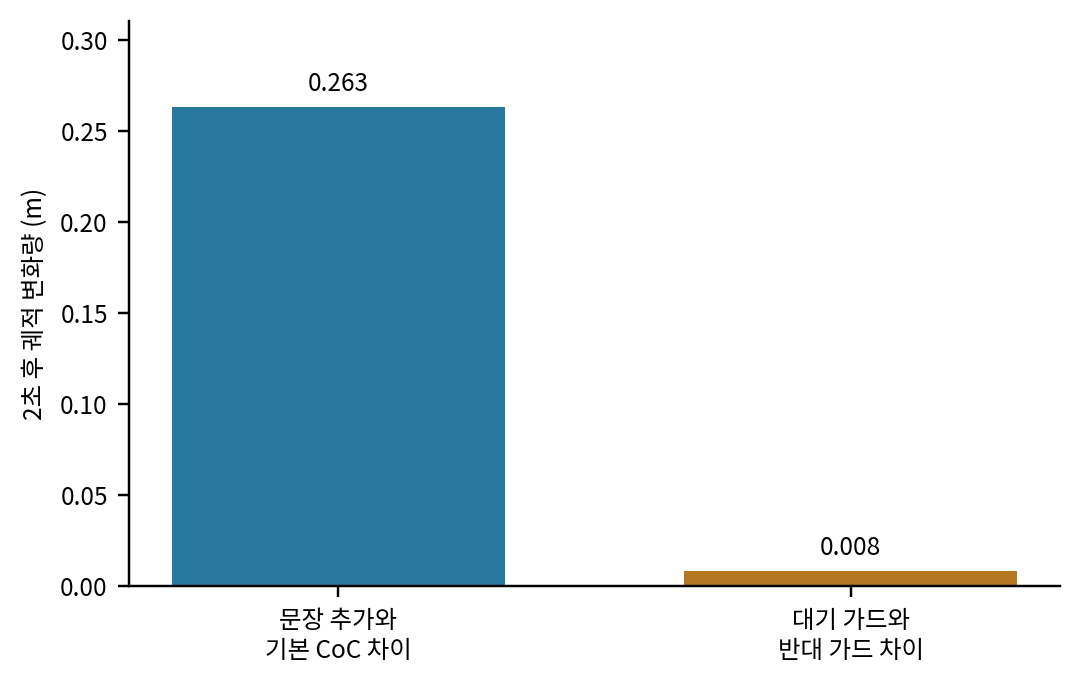
\includegraphics[width=0.94\columnwidth]{figures/fig04_r1_diagnostic.png}
\caption{Alpamayo-R1 사전 진단. 첫 막대는 문장을 추가했을 때 기본 CoC에서 궤적이 얼마나 달라졌는지를, 두 번째 막대는 서로 반대되는 두 가드 사이에서 궤적이 얼마나 달라졌는지를 나타낸다.}
\label{fig:r1-diagnostic}
\end{figure}

\subsection{최소 가드-행동 학습과 초기 과제의 한계}

\paragraph{확인 목적.}
두 번째 실험은 작은 VLM이 "이 가드에서는 정지하고, 저 가드에서는 진행한다"는 대응을 학습할 수 있는지 확인한다. 동시에 정지와 진행만 구분하는 쉬운 문제가 가드의 효과를 실제보다 크게 보이게 할 수 있는지도 확인한다.

\paragraph{비교 방법.}
후보는 정지(STOP)와 진행(PROCEED) 두 가지로 만들었다. 첫 조건에서는 가드와 정답 행동을 올바르게 연결했다. 비교 조건에서는 같은 가드 문장을 사용하되 정답 행동과의 연결을 일부러 섞었다. 이 비교를 통해 모델이 단순히 문장을 받은 효과와 가드의 올바른 의미를 배운 효과를 구분한다. 평가는 학습에 사용하지 않은 장면과, 같은 뜻을 다른 문장으로 표현한 경우로 나누었다. 쉬운 과제에서는 학습량의 차이가 결과에 영향을 주지 않도록 기존 CoC와 CoC+Guard의 학습 횟수도 같게 맞추었다.

\paragraph{결과.}
학습에 사용하지 않은 장면에서 올바른 가드 대응 조건의 정확도는 0.990, 쌍 정확도는 0.958이었다. 반면 대응을 섞은 조건은 각각 0.719와 0.000이었다. 이는 올바른 가드--행동 관계를 학습하면 새로운 장면에서도 두 가드를 구별할 수 있음을 보여준다. 그러나 같은 뜻을 다른 문장으로 바꾼 평가에서는 두 조건의 정확도가 0.740과 0.745였고, 쌍 정확도는 모두 0이었다. 즉, 학습한 문장과 비슷한 표현에는 잘 대응했지만 새로운 표현까지 이해하지는 못했다.

또한 학습 자료가 충분한 쉬운 과제에서는 기존 CoC만 사용해도 정확도 0.974와 쌍 정확도 0.896에 도달했고, CoC+Guard는 1.000과 1.000이었다. 학습 횟수를 같게 맞춘 사후 비교에서는 두 조건 모두 1.000이었다.

\paragraph{의미.}
두 가지를 알 수 있다. 첫째, 작은 VLM은 가드와 행동의 관계를 학습할 수 있다. 둘째, 쉬운 정지/진행 문제에서는 가드가 없어도 장면만 보고 정답을 외울 수 있다. 이 경우 CoC+Guard의 높은 정확도가 정말 가드를 읽은 결과인지 분명하지 않다. 따라서 다음 실험부터는 모든 후보가 같은 CoC 목표를 달성하게 만들고, 가드를 지키는지와 얼마나 원활하게 진행하는지만 다르게 구성한다.

\begin{table*}[!t]
\centering
\caption{주요 실험의 비교 대상, 대표 결과 및 의미.}
\label{tab:suite}
\scriptsize
\begin{tabularx}{\textwidth}{L{0.14\textwidth}L{0.19\textwidth}L{0.20\textwidth}L{0.20\textwidth}Y}
\toprule
실험 & 주요 비교 & 핵심 측정값 & 대표 결과 & 의미 \\
\midrule
R1 사전 진단 & 기본 CoC, 대기 가드, 반대 가드 & 2초 후 궤적 변화량 & 기본 CoC와 0.263 m 차이, 반대 가드끼리는 0.008 m 차이 & 문장에는 반응하지만 반대 의미를 구별하지 못함 \\
최소 학습 & 올바른 가드 대응, 대응을 섞은 가드 & 새 장면 정확도, 쌍 정확도 & 올바른 대응 0.990/0.958, 섞은 대응 0.719/0.000 & 가드-행동 관계는 배우지만 새로운 표현에는 약함 \\
정적 후보 & 요구사항 전용형과 네 가드 표현 & 위반률, 보수 선택률, 쌍 정확도 & CoC 통합형: 위반 0.000, 쌍 정확도 1.000 & 같은 목표의 후보 중 가드에 맞는 선택이 가능 \\
시간 조건 & 대기시간이 다른 두 계약 & 가드 위반, 목표 완료, 쌍 정확도 & 요구사항 전용형 위반 0.319, CoC 통합형 0.000 & 대기와 해제 조건을 학습해 선택을 바꿀 수 있음 \\
다중 주행 & 정지, 차선 변경, 어려운 표현 & 위반률, 목표 완료, 쌍 정확도 & 일반 평가 위반 0.000, 어려운 표현 평가 0.010 & 효과가 여러 행동으로 확장되지만 단위 변환 오류가 남음 \\
폐루프 보조 & 상태, CoC, 상황에 따라 바뀌는 계약, 차단장치 & 가드 위반, 충돌, 개입 횟수 & 재위험 상황 위반 46.6\%에서 21.4\%, 차단장치 사용 시 4.8\% & 학습된 계약만으로 부족하며 최신 상태를 이용한 실행 검사가 필요 \\
\bottomrule
\end{tabularx}
\end{table*}

\subsection{동일 목표를 달성하는 정적 궤적 후보}

\paragraph{확인 목적.}
이 실험에서는 모든 후보가 "교차로를 통과한다"는 같은 목표를 달성한다. 따라서 모델은 목표 달성 여부만으로 정답을 고를 수 없다. 현재 가드가 어느 후보를 허용하는지 읽어야 한다.

\paragraph{비교 방법.}
두 후보 모두 교차로를 통과하지만 최대 속도, 장애물과의 최소거리, 진입 시점과 진행 속도가 다르다. 같은 장면에서 완화 계약은 더 빠른 후보를 허용하지만, 엄격 계약은 그 후보를 금지하고 더 신중한 후보를 허용한다. 요구사항 전용형, CoC 통합형, 가드 분리형, 대응을 섞은 가드와 논리식 가드를 비교하였다. 두 계약의 정답을 모두 맞혀야 하는 쌍 정확도를 핵심 지표로 사용하였다.

\begin{table*}[!t]
\centering
\caption{같은 CoC 목표를 달성하는 정적 후보의 분리 평가 결과.}
\label{tab:static}
\footnotesize
\begin{tabular}{lccccc}
\toprule
조건 & 후보 정확도 & 가드 위반 $\downarrow$ & 과도한 보수 $\downarrow$ & 쌍 정확도 $\uparrow$ & 목표 완료 \\
\midrule
요구사항 전용형 & 0.500 & 0.500 & 0.500 & 0.000 & 1.000 \\
CoC 통합형 & \textbf{1.000} & \textbf{0.000} & \textbf{0.000} & \textbf{1.000} & 1.000 \\
가드 분리형 & 0.993 & 0.014 & 0.000 & 0.986 & 1.000 \\
대응을 섞은 가드 & 0.465 & 0.375 & 0.694 & 0.153 & 1.000 \\
논리식 가드 & \textbf{1.000} & \textbf{0.000} & \textbf{0.000} & \textbf{1.000} & 1.000 \\
\bottomrule
\end{tabular}
\end{table*}

\paragraph{결과.}
표~\ref{tab:static}에서 모든 조건의 목표 완료율은 1.000이었다. 즉, 어느 조건도 교차로 통과 자체를 포기하지 않았다. 그러나 가드가 없는 요구사항 전용형은 선택의 절반에서 가드를 위반하여 위반률이 0.500이었고, 두 계약을 모두 맞힌 쌍은 없어 쌍 정확도가 0.000이었다. 대응을 섞은 조건의 쌍 정확도도 0.153에 머물렀다.

반면 CoC 통합형과 논리식 가드는 위반률 0.000, 과도한 보수 선택률 0.000, 쌍 정확도 1.000을 기록하였다. 가드 분리형도 위반률 0.014와 쌍 정확도 0.986으로 높았다. 이 조건들은 같은 장면에서도 계약이 바뀌면 정답 후보를 함께 바꾸었다.

문장을 바꾸어 쓴 평가의 정확도와 쌍 정확도는 CoC 통합형 0.875/0.750, 가드 분리형 0.924/0.847, 논리식 가드 1.000/1.000이었다. 학습하지 않은 수치를 사용한 평가는 각각 1.000/1.000, 0.951/0.903, 0.924/0.847이었다.

\paragraph{의미.}
CoC 통합형은 항상 정지하는 방법으로 위반을 피한 것이 아니다. 모든 후보가 목표를 완료했고, 그중 현재 계약이 허용하는 가장 원활한 후보를 골랐다. 따라서 이 결과는 모델이 실행 가드를 후보 선택에 사용했음을 보여준다. 다만 정적 과제에서 논리식 가드가 높은 성능을 보였다는 이유만으로 논리 표현이 언제나 더 좋다고 결론 내릴 수는 없다. 다음 시간 과제에서는 다른 결과가 나타난다.

\subsection{정지-대기-해제-출발 시간 조건}

\paragraph{확인 목적.}
앞 실험은 속도나 거리처럼 한 시점의 기준을 다루었다. 이번 실험은 "얼마나 오래 기다려야 하며 언제 출발해도 되는가"라는 시간 조건도 모델이 배울 수 있는지 확인한다.

\paragraph{비교 방법.}
장면과 네 후보는 그대로 두고, 상충 구역이 비어 있는 것을 확인한 뒤 기다려야 하는 시간만 바꾸었다. 완화 계약은 짧게 기다린 뒤 출발하는 후보를 허용하고, 엄격 계약은 더 오래 기다린 후보만 허용한다. 후보는 조기 진입, 짧은 대기 후 진입, 긴 대기 후 진입과 계속 정지로 구성하였다. 결과가 학습의 무작위성에 좌우되는지 확인하기 위해 요구사항 전용형과 네 가지 가드 표현을 서로 다른 초기값 42, 17, 123으로 각각 학습하였다.

\begin{table*}[!t]
\centering
\caption{정지-대기-해제-출발 시간 조건의 3회 반복 평균과 표준편차.}
\label{tab:temporal}
\footnotesize
\begin{tabular}{lccccc}
\toprule
조건 & 후보 정확도 & 가드 위반 $\downarrow$ & 교착 $\downarrow$ & 가드 준수 목표 완료 $\uparrow$ & 쌍 정확도 $\uparrow$ \\
\midrule
요구사항 전용형 & $0.500\pm0.000$ & $0.319\pm0.052$ & $0.000\pm0.000$ & $0.681\pm0.052$ & $0.000\pm0.000$ \\
CoC 통합형 & $\mathbf{1.000\pm0.000}$ & $\mathbf{0.000\pm0.000}$ & $0.000\pm0.000$ & $\mathbf{1.000\pm0.000}$ & $\mathbf{1.000\pm0.000}$ \\
가드 분리형 & $0.698\pm0.094$ & $0.191\pm0.136$ & $0.000\pm0.000$ & $0.809\pm0.136$ & $0.396\pm0.187$ \\
대응을 섞은 가드 & $0.510\pm0.015$ & $0.333\pm0.023$ & $0.000\pm0.000$ & $0.667\pm0.023$ & $0.021\pm0.029$ \\
논리식 가드 & $0.538\pm0.027$ & $0.274\pm0.108$ & $0.000\pm0.000$ & $0.726\pm0.108$ & $0.076\pm0.055$ \\
\bottomrule
\end{tabular}
\end{table*}

\paragraph{결과.}
표~\ref{tab:temporal}과 그림~\ref{fig:temporal-pair}(a)에서 CoC 통합형은 세 번의 반복 모두 가드 위반 0.000, 가드 준수 목표 완료 1.000, 쌍 정확도 1.000을 기록하였다. 대기시간이 바뀔 때마다 짧은 대기 후보와 긴 대기 후보를 올바르게 바꾼 것이다. 반면 요구사항 전용형의 가드 위반률은 $0.319\pm0.052$였고 쌍 정확도는 0이었다. 가드 분리형은 평균적으로 요구사항 전용형보다 나았지만 초기값에 따라 결과 차이가 컸다. 대응을 섞은 가드와 논리식 가드는 두 대기시간의 차이를 안정적으로 배우지 못했다.

\paragraph{의미.}
CoC 통합형은 단순히 정지와 진행을 구별한 것이 아니다. 같은 장면에서도 가드가 요구하는 대기시간을 읽고 출발 시점을 바꾸었다. 한편 논리식 가드의 낮은 결과는 논리식 자체가 자연어보다 나쁘다는 뜻이 아니다. 기반 VLM이 자연어에는 익숙하지만 현재 사용한 논리 문법에는 충분히 적응하지 못했을 수 있다. 두 표현을 공정하게 비교하려면 논리 문법을 따로 학습시킨 뒤 다시 평가해야 한다.

\subsection{정지·차선 변경과 어려운 표현}

\paragraph{확인 목적.}
앞 실험의 성공이 대기시간 문제에만 나타난 결과일 수 있다. 이를 확인하기 위해 정지와 차선 변경으로 행동을 넓혔다. 또한 같은 가드를 다른 문장이나 처음 보는 수치로 표현해도 모델이 조건을 지키는지 확인하였다.

\paragraph{비교 방법.}
정지 과제에서는 정지선 위치, 최대 감속도와 최대 가가속도를 가드로 사용하였다. 차선 변경 과제에서는 최소 차량 간격과 중단 후 재시도 조건을 사용하였다. 192개 장면마다 완화 계약과 엄격 계약을 하나씩 적용하여 384개 학습 예를 만들었다. 일반 평가, 같은 뜻을 바꾸어 쓴 문장 평가와 학습하지 않은 수치 평가는 각각 48개 장면, 즉 96개 계약 문제로 구성하였다. 별도의 어려운 표현 평가에는 기준값과 정확히 같은 경우, 부정·금지 문장, 조건문의 순서 변경과 m를 cm로 바꾼 문장을 함께 넣었다.

\begin{table*}[!t]
\centering
\caption{다중 주행 과제의 일반 평가와 어려운 표현 평가 결과. 값은 3회 반복 평균과 표준편차다.}
\label{tab:maneuver}
\footnotesize
\begin{tabular}{llcccc}
\toprule
평가 & 조건 & 후보 정확도 & 가드 위반 $\downarrow$ & 가드 준수 목표 완료 $\uparrow$ & 쌍 정확도 $\uparrow$ \\
\midrule
일반 & 요구사항 전용형 & $0.500\pm0.000$ & $0.292\pm0.072$ & $0.708\pm0.072$ & $0.000\pm0.000$ \\
 & Safety-Constrained CoC & $\mathbf{1.000\pm0.000}$ & $\mathbf{0.000\pm0.000}$ & $\mathbf{1.000\pm0.000}$ & $\mathbf{1.000\pm0.000}$ \\
 & 대응을 섞은 가드 & $0.503\pm0.006$ & $0.267\pm0.039$ & $0.733\pm0.039$ & $0.028\pm0.032$ \\
\midrule
어려운 표현 & 요구사항 전용형 & $0.500\pm0.000$ & $0.302\pm0.065$ & $0.698\pm0.065$ & $0.000\pm0.000$ \\
 & Safety-Constrained CoC & $\mathbf{0.948\pm0.063}$ & $\mathbf{0.010\pm0.010}$ & $\mathbf{0.990\pm0.010}$ & $\mathbf{0.896\pm0.127}$ \\
 & 대응을 섞은 가드 & $0.535\pm0.079$ & $0.260\pm0.018$ & $0.740\pm0.018$ & $0.090\pm0.139$ \\
\bottomrule
\end{tabular}
\end{table*}

\paragraph{결과.}
일반 평가에서 Safety-Constrained CoC는 정지와 차선 변경 모두 가드 위반 0.000, 가드 준수 목표 완료 1.000, 쌍 정확도 1.000을 기록하였다. 즉, 두 행동에서 목표를 완료하면서 완화·엄격 계약의 정답을 모두 바꾸어 골랐다. 요구사항 전용형보다 평균 위반률은 0.292 낮았다. 초기값을 단위로 다시 뽑아 계산한 95\% 구간은 [0.250, 0.375]였다. 대응을 섞은 가드보다 쌍 정확도는 0.972 높았고 해당 구간은 [0.938, 1.000]이었다. 다만 학습을 세 번만 반복했으므로 이 구간은 확정적인 통계 결론이 아니라 결과의 범위를 살펴보는 참고값이다.

어려운 표현 평가에서는 가드 위반률이 $0.010\pm0.010$, 쌍 정확도가 $0.896\pm0.127$로 낮아졌다. 오답 15개는 모두 같은 거리를 m 대신 cm로 표현한 문장에서 발생하였다. 초기값 42에서 나온 오답 12개는 가드를 어기지는 않았지만 필요 이상으로 느린 차선 변경 후보를 선택한 경우였다. 나머지 3개는 감속도 또는 가가속도 상한을 넘은 정지 후보를 선택한 경우였다. 부정 표현, 조건문의 순서 변경과 m 단위 경계값만 포함한 예에서는 오답이 없었다.

\paragraph{의미.}
가드를 CoC 안에 함께 제시하는 효과는 대기시간뿐 아니라 정지와 차선 변경에서도 나타났다. 그러나 단위를 바꾼 문장에서는 오류가 남았다. 이번 어려운 표현 평가에는 여러 변화가 함께 포함되었으므로, 모든 오류의 원인이 단위 변환이라고 확정할 수는 없다. 후속 실험에서는 단위, 부정 표현, 조건 순서와 경계값을 한 번에 하나씩만 바꾸어 원인을 분리해야 한다.

\begin{figure*}[!t]
\centering
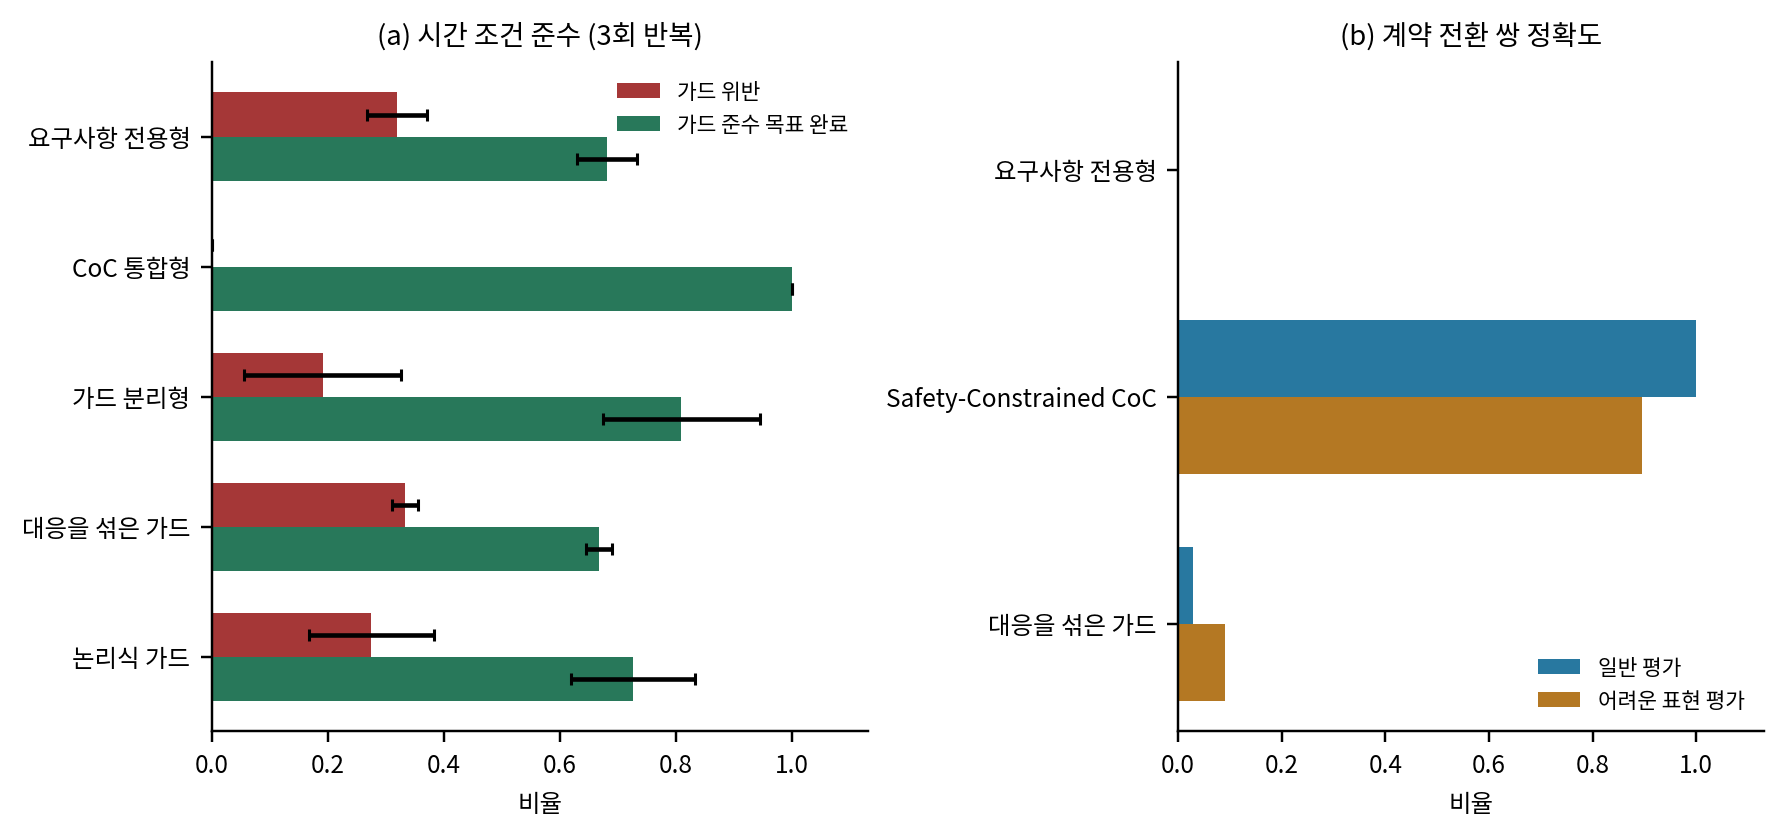
\includegraphics[width=0.98\textwidth]{figures/fig05_temporal_pair.png}
\caption{시간 조건과 다중 주행 과제의 결과. (a)는 시간 조건별 가드 위반률과 가드 준수 목표 완료율, (b)는 일반 평가와 어려운 표현 평가의 계약 전환 쌍 정확도를 비교한다. 오차 막대는 3회 반복의 표준편차다.}
\label{fig:temporal-pair}
\end{figure*}

\subsection{폐루프 보조 실험}

\paragraph{확인 목적.}
앞의 실험은 VLM이 미리 주어진 후보를 한 번 선택하는 문제였다. 마지막 실험은 선택 뒤에도 상황이 계속 바뀌는 경우를 살펴본다. 학습된 계약만 사용할 때와, 실행 중 위험한 명령을 막는 차단 장치를 함께 사용할 때를 비교한다. 이 실험은 작은 신경망과 단순한 운동 모델을 사용한 보조 분석이며, 앞의 VLM 결과나 실제 차량과 직접 비교하지 않는다.

\paragraph{비교 방법.}
두 층 신경망과 1차원 운동학으로 만든 소규모 폐루프 환경을 사용하였다. 폐루프란 모델이 한 번만 답하는 것이 아니라, 매 시점의 상태를 다시 받아 다음 행동을 계속 정하는 환경을 뜻한다. 상태만 주는 조건, 상태와 CoC를 주는 조건, 상황에 따라 바뀌는 동적 계약, 한 번 진행으로 바뀌면 다시 대기로 돌아가지 않는 단조 단계 계약과 계약+차단장치를 비교하였다.

평가는 두 상황으로 나누었다. 첫째, 학습 자료에 정지, 대기, 출발 등 모든 주행 단계가 충분히 들어 있는 상황이다. 둘째, 출발이 허용된 뒤 다른 차량이 다시 나타나므로 다시 정지해야 하지만 학습에서는 보지 못한 "해제 후 위험 재등장" 상황이다. 앞으로 1.2초의 모든 상황을 미리 아는 조건도 넣었지만, 이는 실제 방법이 아니라 도달 가능한 가장 좋은 결과를 보기 위한 참고값이다.

\begin{figure*}[!t]
\centering
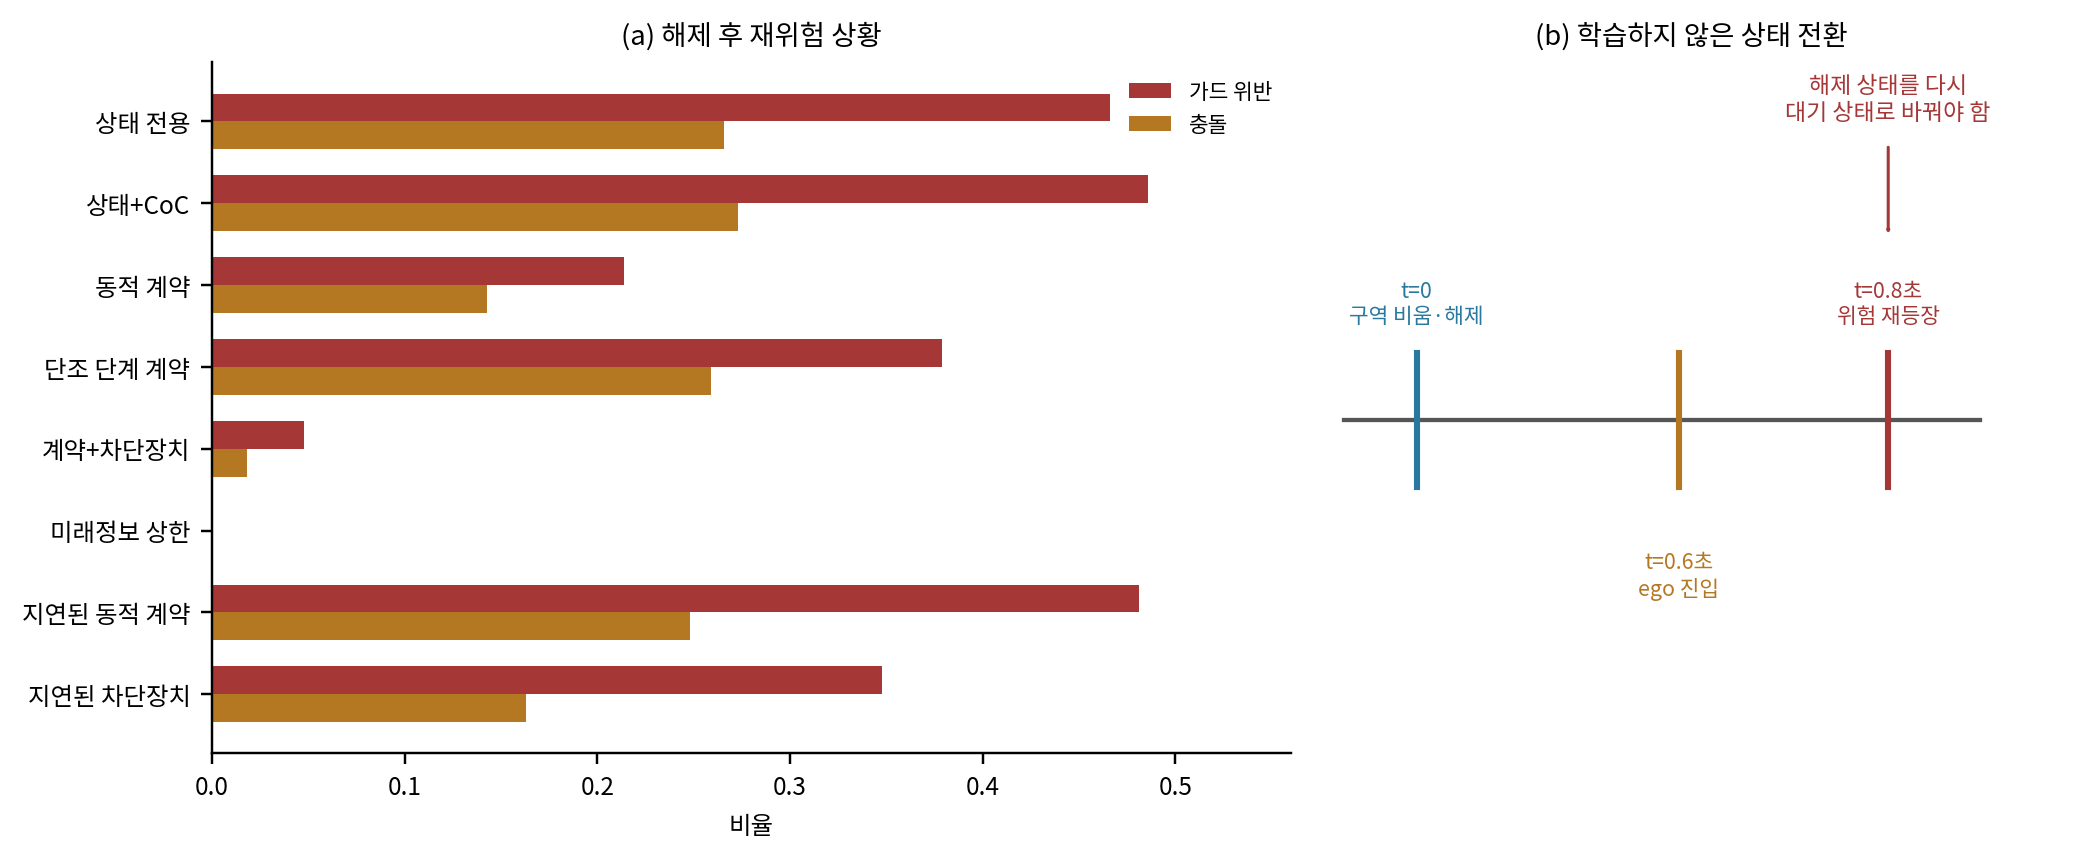
\includegraphics[width=0.98\textwidth]{figures/fig06_release_reversal.png}
\caption{폐루프 보조 실험. (a)는 출발이 허용된 뒤 위험이 다시 나타나는 상황에서 각 방법의 가드 위반률과 충돌률을 비교한다. (b)는 출발 허용, 다른 차량의 진입, 다시 정지해야 하는 순간의 순서를 보여준다. 미래정보 상한은 앞으로의 상황을 완벽히 안다고 가정한 참고값이며 실제 적용 방법이 아니다.}
\label{fig:release-reversal}
\end{figure*}

\paragraph{결과.}
먼저 모든 주행 단계를 학습한 상황을 보았다. 정지 후 대기로 넘어가는 예 1,404개를 학습 자료에 추가하자 상태 전용, 상태+CoC, 동적 계약과 단조 단계 계약 모두 300회 평가에서 정지 구간에 너무 일찍 들어가지 않았다. 학습 분포 밖 상황의 가드 위반률도 상태 전용 2.6\%, 상태+CoC 1.4\%, 동적 계약, 단조 단계 계약과 계약+차단장치는 모두 0\%였다. 이 경우 차단장치는 위반률을 더 낮추지 못했지만 주행할 때마다 평균 2.539회 개입했다. 이미 학습으로 해결된 상황에서는 차단장치가 불필요하게 작동할 수 있음을 뜻한다.

그러나 그림~\ref{fig:release-reversal}의 해제 후 재위험 상황에서는 결과가 달랐다. 가드 위반률은 상태 전용 46.6\%, 상태+CoC 48.6\%, 동적 계약 21.4\%, 단조 단계 계약 37.9\%, 계약+차단장치 4.8\%였다. 동적 계약은 현재 위험 상태를 알려 주어 위반을 줄였고, 차단장치는 위험한 행동을 실행 직전에 막아 위반을 더 줄였다. 충돌률도 같은 순서로 26.6\%, 27.3\%, 14.3\%, 25.9\%, 1.8\%였다.

모든 조건의 목표 완료율은 100\%였으므로 낮은 위반률이 단순히 차량을 계속 세운 결과는 아니었다. 앞으로의 상황을 완벽히 아는 비현실적 조건만 위반과 충돌이 모두 0\%였다. 또한 계약 정보가 실제 상황보다 0.4초 늦게 도착하면 동적 계약의 위반률은 48.1\%, 계약+차단장치는 34.8\%로 증가하였다. 올바른 계약도 늦게 전달되면 효과가 크게 줄어든다는 뜻이다.

\paragraph{의미.}
충분한 성공 시연이 있으면 모델은 문장에 적히지 않은 일부 제약도 행동 예에서 배울 수 있다. 이때 차단장치를 항상 사용하면 성능을 더 높이지 못하면서 개입만 늘어날 수 있다. 그러나 학습하지 않은 위험이 다시 나타나면 동적 계약만으로는 위반을 모두 막지 못했다. 최신 상태를 사용하는 차단장치를 함께 사용했을 때 위반과 충돌이 가장 크게 줄었다. 그 효과도 계약 정보가 늦으면 감소했다. 따라서 학습된 가드는 도움이 되지만, 새로운 위험과 정보 지연까지 혼자서 해결하지는 못한다.

\flushbottom
\section{논의와 연구 범위}
\label{sec:discussion}

본 장에서는 5장의 결과가 무엇을 뜻하는지, 그리고 그 결과를 어디까지 해석할 수 있는지 설명한다. 핵심은 기본 CoC를 실행 가드로 보완하는 학습과, 실제 실행 단계에서 궤적을 다시 검사하는 일을 구분하는 것이다.

\subsection{기본 CoC와 실행 가드가 맡는 역할}

기본 CoC는 "보행자에게 양보한 뒤 진행한다"처럼 달성할 행동과 그 이유를 설명한다. 실행 가드는 "정지선을 넘지 않는다" 또는 "상충 구역이 1.5초 동안 비어 있을 때만 출발한다"처럼 그 행동을 언제, 어느 범위에서 허용할지를 정한다. Safety-Constrained CoC는 이 두 정보를 한 문맥에 넣은 CoC 통합형이다.

시간 조건 실험에서 요구사항 전용형의 가드 위반률은 0.319였지만 CoC 통합형은 0.000이었다. 이 결과는 기본 CoC가 위험하다는 뜻이 아니다. 기본 CoC에는 짧게 기다릴지 길게 기다릴지를 구분할 정보가 없었고, 실행 가드를 추가했을 때 모델이 그 차이를 배울 수 있었다는 뜻이다. 따라서 본 논문의 기여는 기존 CoC를 부정하는 것이 아니라, CoC가 말하지 않은 허용 조건을 학습 가능한 형태로 보완하는 데 있다.

\subsection{CoC 통합형이 높은 결과를 보인 이유}

시간 조건 실험에서 CoC 통합형은 가드를 분리해서 준 방식이나 논리식으로 준 방식보다 안정적인 결과를 보였다. 한 가지 가능한 이유는 기반 VLM이 자연어 문장에 익숙하고, CoC의 행동 목표와 실행 가드를 한 문맥에서 함께 처리할 수 있기 때문이다. 반대로 가드 분리형은 서로 떨어진 두 정보를 연결해야 하고, 논리식 가드는 모델이 익숙하지 않은 문법을 추가로 배워야 한다.

그러나 이 결과만으로 자연어가 논리식보다 본질적으로 우수하다고 결론 내릴 수는 없다. 정적 후보 실험에서는 논리식 가드도 위반률 0.000과 쌍 정확도 1.000을 기록하였다. 표현 방식을 공정하게 비교하려면 논리 문법을 따로 학습시키고, 각 조건에 같은 양의 학습 자료와 학습 횟수를 제공한 뒤 다시 평가해야 한다. 현재 결과가 직접 보여주는 것은 자연어의 보편적 우수성이 아니라, 현재 VLM과 학습 조건에서는 CoC 통합형이 가장 안정적이었다는 점이다.

\subsection{수치 조건은 독립 검증기가 다시 확인해야 한다}

어려운 표현 평가의 오답 15개는 모두 같은 거리를 m 대신 cm로 표현한 문장에서 발생하였다. 모델은 실행 가드의 일반적인 의미를 배웠지만, 수치와 단위를 바꾸는 계산까지 항상 정확하게 처리하지는 못했다. 따라서 실제 적용에서는 모델에 모든 계산을 맡기지 않고 그림~\ref{fig:future-architecture}과 같이 역할을 나누는 것이 적절하다.

먼저 모델은 자연어 Safety-Constrained CoC에서 행동 목표와 실행 가드의 의미를 읽는다. 다음 단계에서는 "최소 간격 600 cm"를 조건 종류, 비교 방향, 값과 단위로 나눈다. 그 뒤 600 cm를 6.0 m처럼 기준 단위로 통일한다. 마지막으로 독립 검증기 또는 차단장치가 선택한 궤적의 거리, 속도와 시간 조건을 수치로 검사한다.

이 과정에서는 "미만"과 "이하"처럼 경계값 포함 여부를 구분해야 한다. 또한 가드를 지킬 수 없을 때 정지할지, 다시 기다릴지와 같은 대체 행동도 정해야 한다. 모델은 문장의 목표와 조건을 해석하고, 검증기는 정확한 수치 경계를 확인하도록 역할을 나누는 것이다.

\begin{figure}[t]
\centering
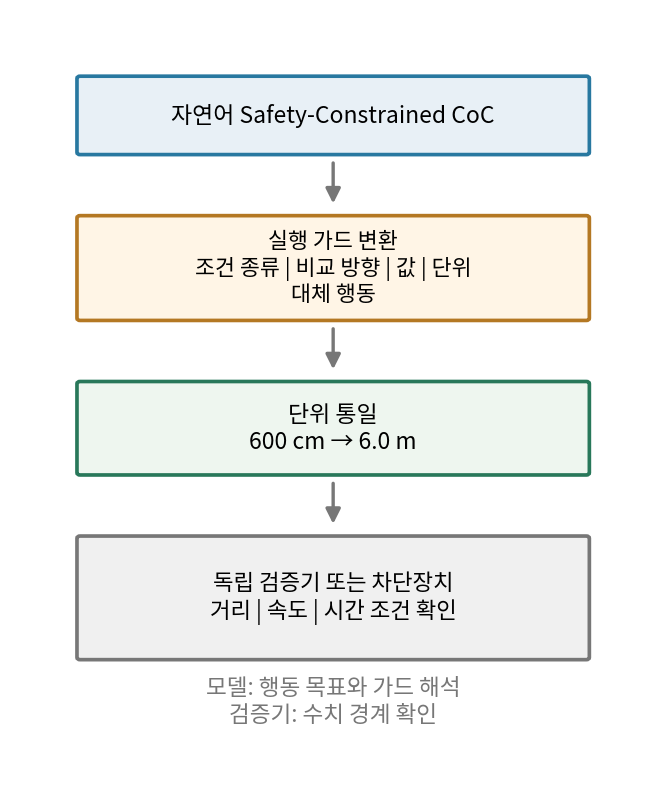
\includegraphics[width=0.94\columnwidth,trim=18 22 18 22,clip]{figures/fig05_typed_contract.png}
\caption{자연어 실행 가드를 실제 검사에 사용하는 네 단계. 모델은 행동 목표와 가드를 해석하고, 독립 검증기 또는 차단장치는 단위를 통일한 수치 조건을 확인한다.}
\label{fig:future-architecture}
\end{figure}

\subsection{학습된 가드와 실행 차단장치는 역할이 다르다}

가드를 학습하면 모델이 가드를 지키는 후보를 선택할 가능성이 높아진다. 그러나 학습에서 보지 못한 모든 상황에서 준수를 보장하지는 않는다. 폐루프의 해제 후 재위험 상황에서 동적 계약은 가드 위반률을 46.6\%에서 21.4\%로 줄였지만 위반을 없애지는 못했다. 최신 상태를 사용하는 차단장치를 함께 적용했을 때 위반률은 4.8\%까지 낮아졌다. 이는 학습된 계약과 실행 단계 검사가 서로 다른 역할을 맡는다는 것을 보여준다.

차단장치도 모든 문제를 해결하지는 못한다. 계약 정보가 0.4초 늦게 도착했을 때 계약+차단장치의 위반률은 34.8\%로 증가하였다. 계약 자체가 틀리거나 중요한 위험이 빠져 있어도 차단장치는 잘못된 조건을 정확하게 집행할 뿐이다. 따라서 실제 시스템에서는 위험이 다시 나타나면 출발 허용을 취소하고 대기 상태로 돌아갈 수 있어야 한다. 계약이 어느 시점의 상황을 설명하는지도 확인해야 하며, 미래 상황이 불확실하면 더 신중한 대체 행동을 선택해야 한다.

\subsection{주 실험이 실제로 확인한 것}

주 실험은 모델이 연속 궤적을 새로 생성하는 문제가 아니다. 합성 이미지와 수치가 적힌 궤적 후보를 주고 그중 하나를 선택하게 한 실험이다. 따라서 이 실험이 직접 확인한 것은 모델이 실행 가드를 읽고 후보 선택을 바꿀 수 있는가이다.

쌍대 계약은 같은 장면에서 가드만 바꾸므로 장면만 보고 같은 답을 반복하는 방법을 막는다. 가드 준수 목표 완료율은 모델이 가드 위반을 피하려고 끝까지 정지하는 방법도 막는다. 이 두 지표를 함께 사용하면 모델이 행동 목표를 끝내면서 가드에 맞는 후보를 골랐는지 확인할 수 있다. 그러나 후보의 물리량과 정답은 연구자가 설계했으며, 실제 차량의 복잡한 움직임이나 모든 충돌 위험을 포함하지 않는다. 그러므로 높은 점수는 제한된 후보 선택 문제에서의 가드 학습 효과이지 실제 차량 안전의 증명이 아니다.

\subsection{결과를 해석할 때의 실험적 한계}

후보 문자를 장면마다 바꾸어 같은 문자만 고르는 암기를 막았고, 대응을 섞은 가드로 문장 추가 자체의 효과를 구분하였다. 또한 학습의 무작위성을 바꾼 세 가지 초기값으로 실험을 반복하였다. 이러한 설계는 가드와 정답 후보의 관계를 실제로 학습했는지 확인하는 데 도움이 된다.

다만 반복 횟수가 세 번으로 적다. 어려운 표현 평가에는 단위 변환, 부정 표현, 경계값과 조건 순서 변경이 함께 들어 있다. 오답이 cm 문장에 집중되었지만, 현재 결과만으로 단위 변환 하나가 모든 오류의 원인이라고 확정할 수는 없다. 후속 실험에서는 장면과 나머지 문장을 고정하고 단위, 부정 표현, 경계값 포함 여부와 복합 조건을 한 번에 하나씩만 바꾸어 각 요인의 영향을 분리해야 한다.

\subsection{Alpamayo-R1과 실제 도로로 확장할 때의 범위}

작은 Qwen VLM의 후보 선택 결과가 Alpamayo-R1의 연속 궤적 생성에서도 그대로 나타난다고 볼 수는 없다. Alpamayo-R1 사전 진단은 모델이 CoC에 추가된 문장에는 반응하지만, 반대되는 가드의 의미를 안정적으로 구별하지 못했다는 결과만 제공한다. Alpamayo-R1에도 같은 효과가 있는지 확인하려면 가드 준수 학습을 직접 수행한 뒤 연속 궤적을 독립 검증해야 한다.

또한 본 논문의 실행 가드는 도로 안전 전체가 아니라 정지선, 최소 간격, 속도와 대기시간 같은 일부 조건만 다룬다. 실제 도로에서는 센서에 보행자나 차량이 실제로 보이는지, 보행자·자전거·차량의 위치와 이동 경로가 어떻게 겹치는지, 선택한 궤적의 충돌 위험은 얼마인지도 확인해야 한다. 계약이 센서의 어느 시점과 대응하는지 기록하고, 사람의 검토나 측정값으로 만든 독립된 정답 자료와 비교하는 평가도 필요하다. 따라서 다음 단계는 작은 VLM 결과를 실제 안전으로 확대 해석하는 것이 아니라, Alpamayo-R1의 연속 궤적과 실제 센서 근거에서 같은 질문을 다시 검증하는 것이다.

\section{결론}
\label{sec:conclusion}

기본 CoC는 주행 장면에서 선택한 행동의 이유와 목표를 설명하지만, 같은 목표를 달성하는 여러 궤적 중 어느 범위까지 허용되는지는 충분히 나타내지 못할 수 있다. 본 논문은 이러한 허용 조건을 보완하기 위해 기본 CoC와 실행 가드를 하나의 문맥으로 결합한 \sccoc{}를 제안하였다. 또한 같은 장면, 행동 목표 및 궤적 후보를 유지한 채 실행 가드만 바꾸는 쌍대 계약 평가를 구성하여, 모델이 장면 유형이나 행동 목표가 아니라 실제 가드의 차이를 읽고 궤적을 선택하는지 확인하였다.

Qwen3-VL-2B-Instruct를 미세 조정한 시간 조건 실험에서 요구사항 전용형 CoC의 가드 위반률은 $0.319\pm0.052$였으나, CoC 통합형에서는 $0.000\pm0.000$으로 감소하였다. 이때 안전한 목표 완료율과 쌍대 계약 정확도는 모두 $1.000$을 유지하여, 위반 감소가 단순히 항상 정지하는 보수적 선택에서 나온 결과가 아님을 확인하였다. 이러한 결과는 정지, 출발 및 차선 변경을 포함한 표준 평가에서도 일관되었다. 다만 어려운 표현 평가에서는 위반률이 $0.010\pm0.010$, 쌍대 계약 정확도가 $0.896\pm0.127$이었고, 오류는 주로 m와 cm처럼 단위 표현이 바뀐 조건에 집중되었다. 따라서 작은 VLM이 행동 목표를 유지하면서 실행 가드를 학습할 수는 있지만, 새로운 수치 표현까지 항상 정확하게 해석한다고 볼 수는 없다.

본 연구의 결과는 합성 장면과 미리 정한 궤적 후보를 사용한 작은 VLM의 선택 실험에 한정되며, Alpamayo-R1의 연속 궤적이나 실제 차량의 안전성을 직접 입증하지 않는다. 보조 폐루프 실험에서도 동적 계약과 차단장치를 함께 사용하면 위반이 줄었지만, 계약 갱신이 늦어지면 다시 증가하여 학습된 가드만으로 안전을 보장할 수 없음을 확인하였다. 실제 적용을 위해서는 자연어 가드를 단위가 표준화된 구조화 조건으로 변환하고, 최신 센서 상태를 이용하는 독립적인 궤적 검증기 및 차단장치와 결합해야 한다. 향후에는 이 구조를 대형 자율주행 VLM의 연속 궤적에 적용하고, 실제 센서 증거와 충돌 위험 지표를 이용해 효과를 검증할 필요가 있다.


\ifieeeclass
  \bibliographystyle{IEEEtran}
\else
  \bibliographystyle{plain}
\fi
\begingroup
\small
\bibliography{references}
\endgroup
\end{document}
